

\section{Experimento BRDF Anisotrópica baseado em Kajiya-Kay (1989)}
\label{section-experiment-kajiya}

Este experimento é baseado no modelo anisotrópico que descreve o comportamento de reflexão de superfícies rugosas simplificadas, proposto no trabalho de Kajiya \cite{kajiya1985anisotropic}. As equações e parâmetros para descrever esse modelo estão na \autoref{fig-kajiya-eqlang-latex}. O código-fonte em \texttt{EquationLang} para o compilador está no \autoref{cod-kajiya-eqlang}. A saída gerada pelo compilador está dividida em duas partes: a parte 1 está no \autoref{cod-kajiya-glsl-pt-1}, enquanto a parte 2 está no \autoref{cod-kajiya-glsl-pt-2}. A renderização dos objetos 3D usando essa BRDF pode ser observada na \autoref{fig-kajiya-objects}. Os \textit{plots} estão presentes na \autoref{fig-kajiya-plots}.

%%%%%%%%%%%%%%%%%%%%%%%%%%%%%%%%%%%%%%%%%%%%%%%%%
\subsection{Representação em documento \LaTeX{}}
%%%%%%%%%%%%%%%%%%%%%%%%%%%%%%%%%%%%%%%%%%%%%%%%%
\begin{figure}[H]
    \caption{\label{fig-kajiya-eqlang-latex} \small Equações da BRDF do experimento baseado em Kajiya-Kay em documento \LaTeX{}.}
    \begin{center}
        % 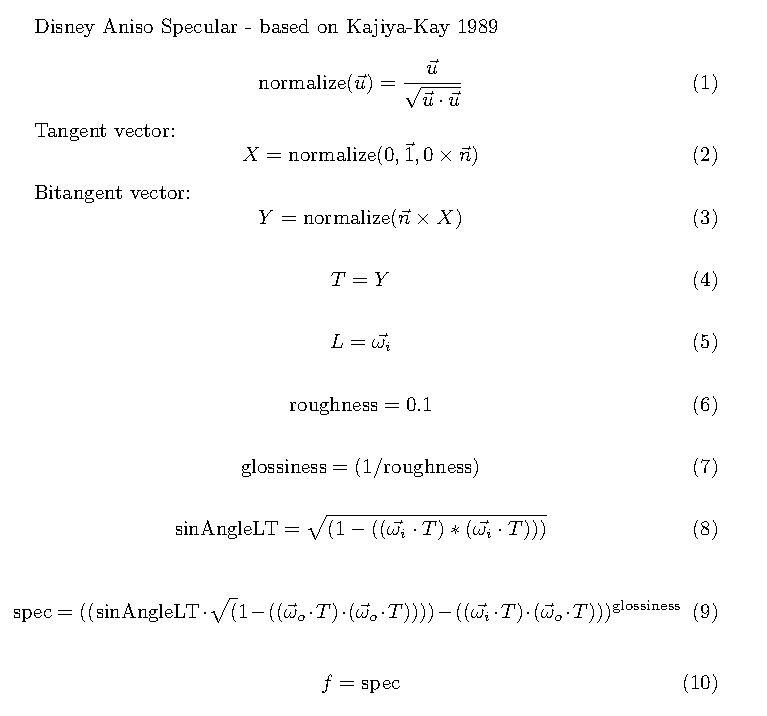
\includegraphics[scale=1.1,width=\textwidth]{./Imagens/brdfs/aniso.pdf}
        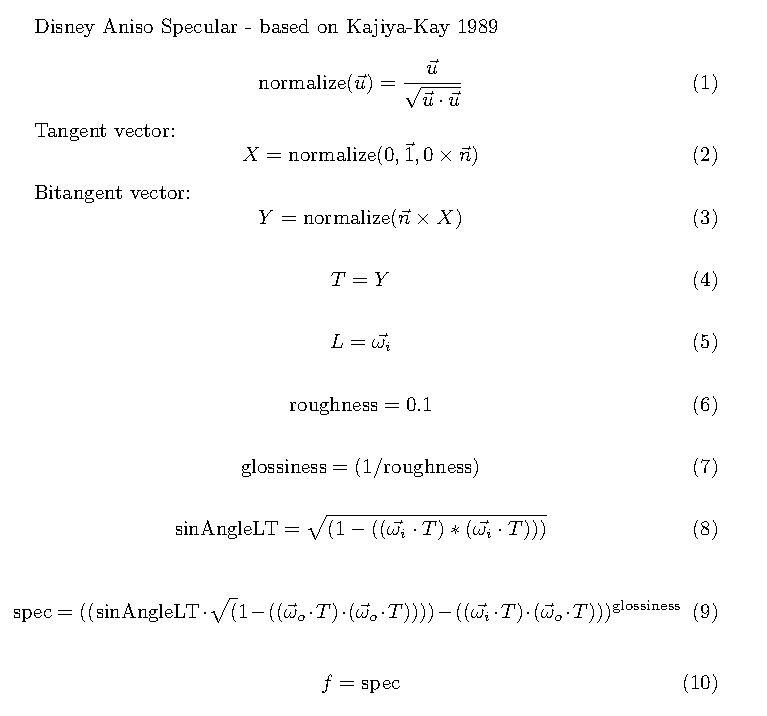
\includegraphics[scale=0.92]{./Imagens/brdfs/aniso.pdf}
    \end{center}
\end{figure}


%%%%%%%%%%%%%%%%%%%%%%%%%%%%%%%%%%%%%%%%%%%%%%%%%
\subsection{Código Fonte em \texttt{EquationLang}}
%%%%%%%%%%%%%%%%%%%%%%%%%%%%%%%%%%%%%%%%%%%%%%%%%
\begin{codigo}[H]
    \caption{\small Código fonte da BRDF do experimento Kajiya-Kay.}
    \label{cod-kajiya-eqlang}
\begin{lstlisting}[language=tex, frame=none, inputencoding=utf8]
Based on Kajiya-Kay 1989

\begin{equation}
  \text{normalize}(\vec{u}) = \frac{\vec{u}}{\sqrt{\vec{u} \cdot \vec{u}}}
\end{equation}

Tangent vector:
\begin{equation}
   X = \text{normalize}(\vec{0,1,0} \times \vec{n})
\end{equation}

Bitangent vector:
\begin{equation}
   Y = \text{normalize}(\vec{n} \times X)
\end{equation}

\begin{equation}
    T = Y
\end{equation}

\begin{equation}
    L = \vec{\omega_i}
\end{equation}

\begin{equation}
    \text{roughness} =  0.1
\end{equation}

\begin{equation}
    \text{glossiness} = (1/\text{roughness})
\end{equation}

\begin{equation}
    s_\alpha = \sqrt{(1 - ((\vec{\omega_i} \cdot T) * (\vec{\omega_i} \cdot T)))}
\end{equation}

\begin{equation}
\text{spec} = ((s_\alpha  \cdot \sqrt(1 - ((\vec \omega_o \cdot T) \cdot (\vec \omega_o \cdot T))))
                  - ((\vec{\omega_i} \cdot T) \cdot (\vec \omega_o \cdot T)))^ \text{glossiness}
\end{equation}
\begin{equation}
f = \text{spec}
\end{equation}
\end{lstlisting}
\end{codigo}
%%%%%%%%%%%%%%%%%%%%%%%%%%%%%%%%%%%%%%%%%%%%%%%%%
\subsection{Código GLSL Gerado}
%%%%%%%%%%%%%%%%%%%%%%%%%%%%%%%%%%%%%%%%%%%%%%%%%
\begin{codigo}[H]
    \caption{\small Saída do compilador: código GLSL da BRDF do experimento baseado em Kajiya-Kay (parte 1 de 2).}
    \label{cod-kajiya-glsl-pt-1}
\begin{lstlisting}[language=C, inputencoding=utf8]
analytic ::begin parameters
#[type][name][min val][max val][default val]
::end parameters
::begin shader
//////////// START OF BUILTINS DECLARTION ////////////
vec3 var_0_vec_h;
vec3 var_3_vec_n;
float var_10_theta_h;
float var_11_theta_d;
float var_1_pi;
float var_2_epsilon;
vec3 var_4_vec_omega_i;
float var_5_theta_i;
float var_6_phi_i;
vec3 var_7_vec_omega_o;
float var_8_theta_o;
float var_9_phi_o;
//////////// END OF BUILTINS DECLARTION ////////////

//////////// START OF USER DECLARED ////////////
vec3 var_12_L;
vec3 var_15_X;
vec3 var_16_Y;
vec3 var_17_T;
float var_18_s_alpha;
float var_19_text_roughness;
float var_20_text_glossiness;
float var_21_text_spec;
float var_22_f;
//////////// END OF USER DECLARED ////////////
//////////// START FUNCTIONS DECLARATIONS ////////////
vec3 var_13_text_normalize(vec3 var_14_vec_u) {
  return (var_14_vec_u / sqrt(dot(var_14_vec_u, var_14_vec_u)));
}
//////////// END FUNCTIONS DECLARATIONS ////////////
\end{lstlisting}
\end{codigo}

\begin{codigo}[H]
    \caption{\small Saída do compilador: código GLSL da BRDF do experimento baseado em Kajiya-Kay (parte 2 de 2).}
    \label{cod-kajiya-glsl-pt-2}
\begin{lstlisting}[language=C, inputencoding=utf8]
vec3 BRDF(vec3 L, vec3 V, vec3 N, vec3 X, vec3 Y) {
  //////////// START OF BUILTINS INITIALIZATION ////////////
  var_0_vec_h = normalize(L + V);
  var_3_vec_n = normalize(N);
  var_1_pi = 3.141592653589793;
  var_2_epsilon = 1.192092896e-07;
  var_4_vec_omega_i = L;
  var_5_theta_i = atan(var_4_vec_omega_i.y, var_4_vec_omega_i.x);
  var_6_phi_i = atan(sqrt(var_4_vec_omega_i.y * var_4_vec_omega_i.y +
                          var_4_vec_omega_i.x * var_4_vec_omega_i.x),
                     var_4_vec_omega_i.z);
  var_7_vec_omega_o = V;
  var_8_theta_o = atan(var_7_vec_omega_o.y, var_7_vec_omega_o.x);
  var_9_phi_o = atan(sqrt(var_7_vec_omega_o.y * var_7_vec_omega_o.y +
                          var_7_vec_omega_o.x * var_7_vec_omega_o.x),
                     var_7_vec_omega_o.z);
  var_10_theta_h = acos(dot(var_0_vec_h, N));
  var_11_theta_d = acos(dot(var_0_vec_h, var_4_vec_omega_i));
  //////////// END OF BUILTINS INITIALIZATION ////////////
  var_12_L = var_4_vec_omega_i;
  var_15_X = var_13_text_normalize(cross(vec3(0.0, 1.0, 0.0), var_3_vec_n));
  var_16_Y = var_13_text_normalize(cross(var_3_vec_n, var_15_X));
  var_17_T = var_16_Y;
  var_18_s_alpha = sqrt(((1.0 - (((dot(var_4_vec_omega_i, var_17_T)) *
                                  (dot(var_4_vec_omega_i, var_17_T)))))));
  var_19_text_roughness = 0.1;
  var_20_text_glossiness = ((1.0 / var_19_text_roughness));
  var_21_text_spec =
      pow(((((var_18_s_alpha *
              sqrt(((1.0 - (((dot(var_7_vec_omega_o, var_17_T)) *
                             (dot(var_7_vec_omega_o, var_17_T))))))))) -
            (((dot(var_4_vec_omega_i, var_17_T)) *
              (dot(var_7_vec_omega_o, var_17_T)))))),
          var_20_text_glossiness);
  var_22_f = var_21_text_spec;

  return vec3(var_22_f);
}


\end{lstlisting}
\end{codigo}

%%%%%%%%%%%%%%%%%%%%%%%%%%%%%%%%%%%%%%%%%%%%%%%%%
\subsection{Visualização do Resultado}
%%%%%%%%%%%%%%%%%%%%%%%%%%%%%%%%%%%%%%%%%%%%%%%%%

\begin{figure}[H]
    \caption{\small{\textit{Plots} da distribuição de reflexão especular e difusa do experimento baseado em Kajiya-Kay.}}
    \label{fig-kajiya-plots}
\minipage{0.48\textwidth}
    \vspace{42px}
  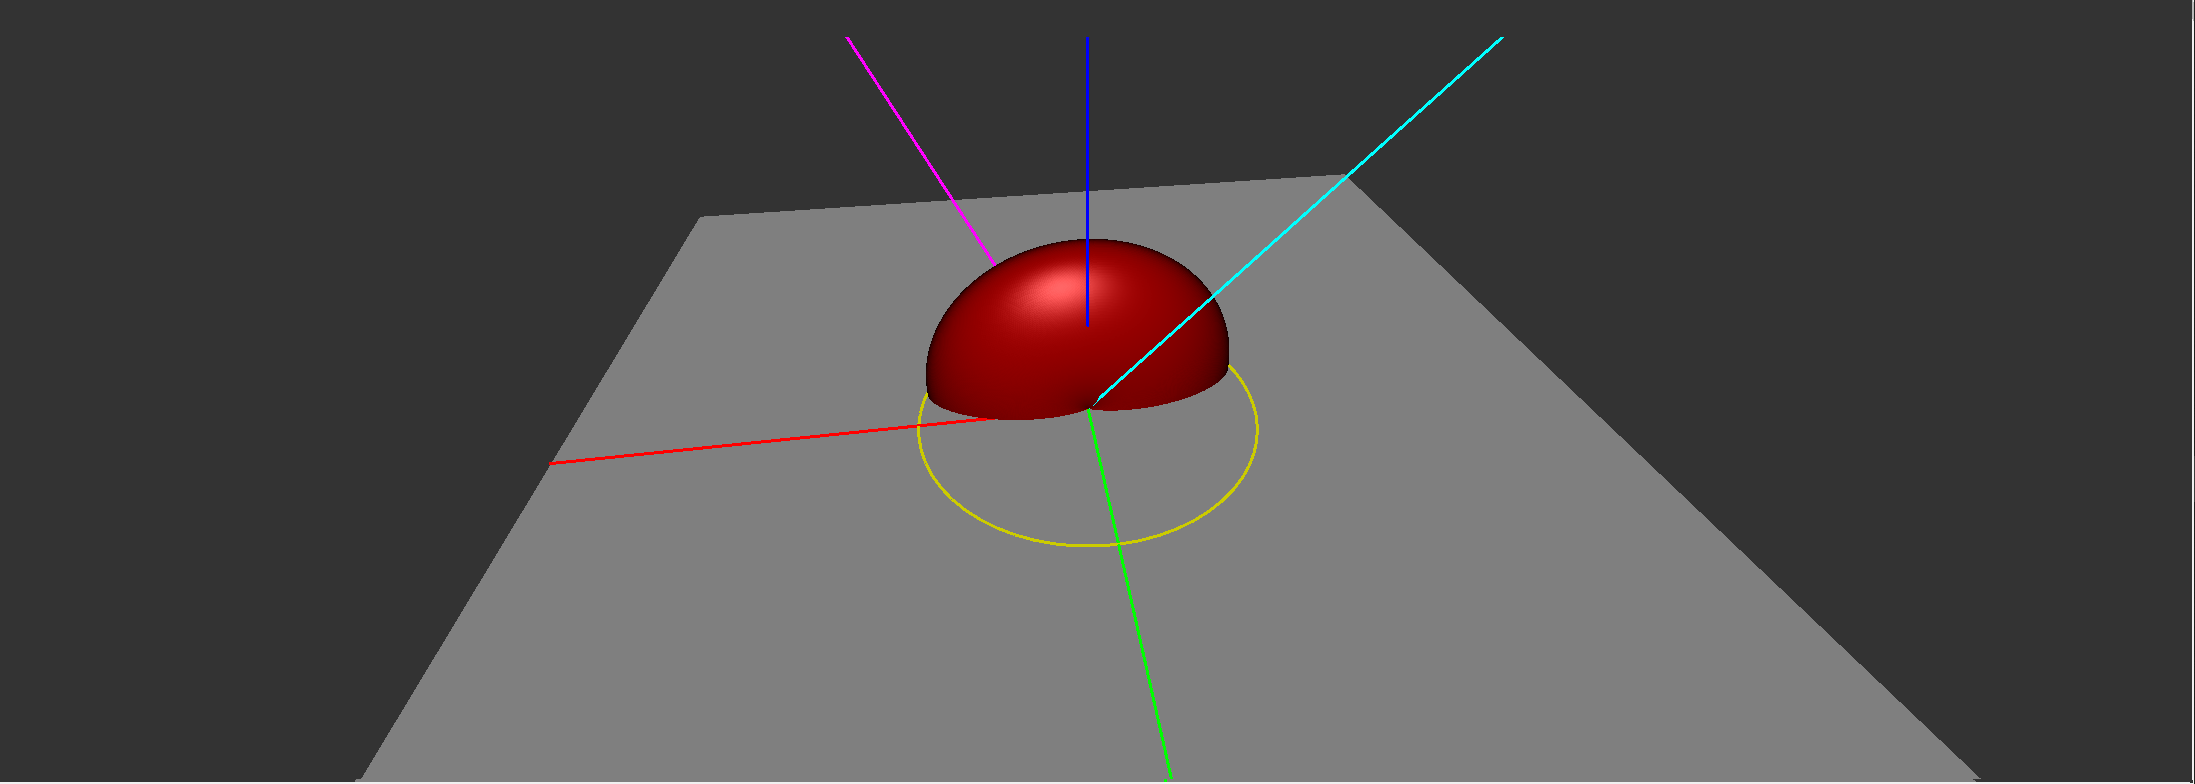
\includegraphics[width=\linewidth]{./Imagens/brdfs/aniso-3D-plot}
    % \caption{\small{(a)}}\label{fig:awesome_image1}
    % \vspace{0.1px}
    \legend{ \small (a) 3D \textit{plot}}
\endminipage\hfill
\minipage{0.48\textwidth}
  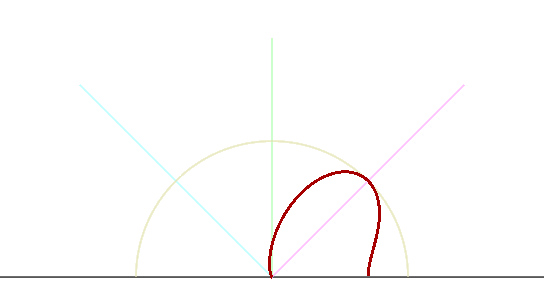
\includegraphics[width=\linewidth]{./Imagens/brdfs/aniso-polar-plot.png}
    \legend{ \small (b) \textit{Polar plot}}
    % \caption{\small{(b)}}\label{fig:awesome_image1}
\endminipage\hfill
\end{figure}

\begin{figure}[H]
    % \caption{\small{Objetos 3D renderizado pelo código GLSL gerado o experimento BRDF Anisotrópica: Kajiya-Kay (1989)}}\label{fig-kajiya-eqlang}
    \caption{\small{Objetos 3D renderizados pelo experimento baseado em Kajiya-Kay.}}
    \label{fig-kajiya-objects}
\minipage{0.32\textwidth}
  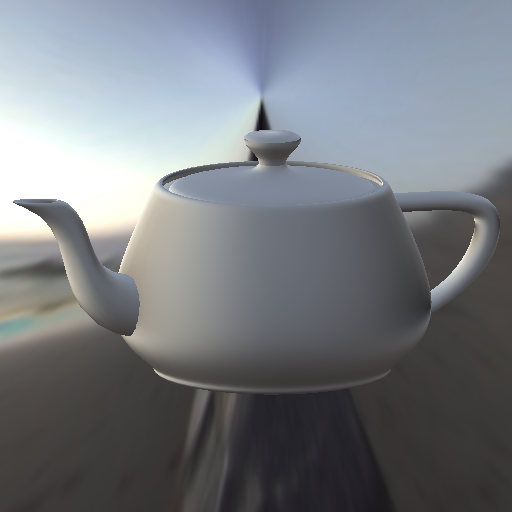
\includegraphics[width=\linewidth]{./Imagens/brdfs/aniso-teapot.png}
    % \caption{\small{(a)}}\label{fig:awesome_image1}
    \legend{ \small (a) \textit{Teapot}}
\endminipage\hfill
\minipage{0.32\textwidth}
  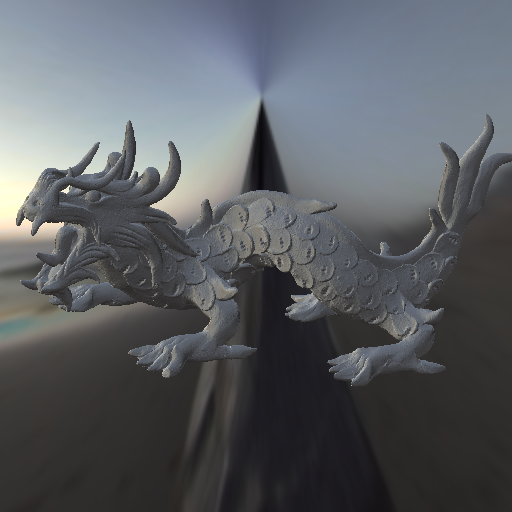
\includegraphics[width=\linewidth]{./Imagens/brdfs/aniso-dragon.png}
    \legend{ \small (b) Dragão de Stanford}
    % \caption{\small{(b)}}\label{fig:awesome_image1}
\endminipage\hfill
\minipage{0.32\textwidth}%
  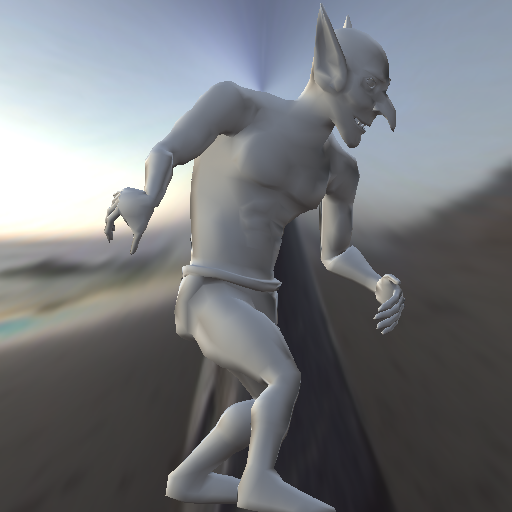
\includegraphics[width=\linewidth]{./Imagens/brdfs/aniso-goblin.png}
    \legend{ \small (c) Goblin}
    % \caption{\small{(c)}}\label{fig:awesome_image1}
\endminipage
\end{figure}

